\documentclass[12pt,a4paper]{report}

\usepackage[margin=1in]{geometry}
\usepackage{graphicx}
\usepackage{array}
\usepackage{booktabs}
\usepackage{longtable}
\usepackage{enumitem}
\usepackage{setspace}
\usepackage{hyperref}
\usepackage{titlesec}
\usepackage{float}
\usepackage{tikz}
\usepackage{listings}
\usepackage{xcolor}
\usepackage{caption}

\usetikzlibrary{positioning,shapes.geometric,arrows.meta}

\hypersetup{
  colorlinks=true,
  linkcolor=black,
  urlcolor=blue,
  pdftitle={DBS Lab Mini Project Report},
  pdfauthor={Harsh Mahesh Kumar and Man Mohit Kumar}
}

\definecolor{codebg}{RGB}{248,248,248}
\definecolor{codeline}{RGB}{220,220,220}

\lstdefinestyle{sqlstyle}{
  basicstyle=\ttfamily\small,
  backgroundcolor=\color{codebg},
  frame=single,
  rulecolor=\color{codeline},
  breaklines=true,
  columns=fullflexible,
  keepspaces=true,
  showstringspaces=false,
  tabsize=2
}

\lstset{style=sqlstyle}

\setstretch{1.25}
\setlength{\parindent}{0pt}
\setlength{\parskip}{0.6em}
\titleformat{\chapter}[display]
  {\normalfont\bfseries\Large}
  {CHAPTER \thechapter}{0.5em}{\Large}

\newcommand{\pk}[1]{\underline{#1}}

\begin{document}

\pagenumbering{gobble}

\begin{titlepage}
  \centering
  
\includegraphics[width=\textwidth]{manipalHeader.png}\par
  \vspace{1.8cm}
  {\bfseries\LARGE DATABASE SYSTEMS LAB MINI PROJECT REPORT\par}
  \vspace{1.2cm}
  {\Large Oracle-Based Student Performance Management System\par}
  \vspace{1.8cm}
  {\large Submitted in partial fulfillment of the requirements for the course Database Systems Lab\par}
  \vfill
  \begin{tabular}{|p{0.42\textwidth}|p{0.18\textwidth}|p{0.22\textwidth}|p{0.12\textwidth}|}
    \hline
    \textbf{Name} & \textbf{Roll No.} & \textbf{Reg No.} & \textbf{Class} \\
    \hline
    Harsh Mahesh Kumar & 23 & 240953320 & CCE-A \\
    \hline
    Man Mohit Kumar & 32 & 240953402 & CCE-A \\
    \hline
  \end{tabular}
  \vfill
  {\large Department of Computer Science and Engineering\par}
  {\large Manipal Institute of Technology, Manipal\par}
  \vspace{0.8cm}
\end{titlepage}

\pagenumbering{roman}

\chapter*{Certificate}
\addcontentsline{toc}{chapter}{Certificate}
This is to certify that the mini project entitled \textit{Oracle-Based Student Performance Management System} has been successfully completed by Harsh Mahesh Kumar (Roll No. 23, Reg No. 240953320, CCE-A) and Man Mohit Kumar (Roll No. 32, Reg No. 240953402, CCE-A) in partial fulfillment of the requirements of Database Systems Lab.

\vspace{2cm}
\begin{flushright}
Faculty Coordinator\\
Department of Computer Science and Engineering\\
Manipal Institute of Technology, Manipal
\end{flushright}

\chapter*{Abstract}
\addcontentsline{toc}{chapter}{Abstract}
The project designs and implements a database-driven student performance system on Oracle DBMS. The system stores students, faculty, courses, course offerings, assessments, marks, grade cutoffs, and semester GPA records. It supports a dynamic assessment structure, so assessment components can be added or changed without redesigning the schema. Weighted totals are derived through SQL aggregation, final grades are resolved from course-specific cutoffs, and data integrity is enforced through database constraints, triggers, functions, procedures, and views. The implementation also exposes student and faculty dashboards through derived views, making the database the single source of truth for academic progress.

\tableofcontents
\listoftables
\clearpage

\pagenumbering{arabic}

\chapter{Introduction}
The project is a course performance management system built around an Oracle relational schema. It models the academic workflow from course offering creation to assessment marking, final grade assignment, and semester GPA tracking. The database is not limited to a fixed number of assignments or exams; instead, every course offering can define its own set of assessment components and grade cutoffs.

The implemented application uses Oracle SQL and PL/SQL to support the following behavior:
\begin{itemize}[leftmargin=1.5em]
  \item storing student, faculty, course, offering, assessment, attempt, attendance, cutoff, and SGPA records,
  \item computing weighted totals from assessment attempts,
  \item assigning grades from dynamically configurable cutoff ranges,
  \item rejecting invalid marks and invalid assessment-weight combinations at the database layer,
  \item generating course and class performance reports through views and procedures.
\end{itemize}

The frontend workspace uses the database through Oracle queries and derived views such as \texttt{v\_student\_course\_progress} and \texttt{v\_student\_profile}. This ensures the report reflects the actual implementation rather than a purely theoretical design.

\chapter{Problem Statement and Objectives}

\section{Problem Statement}
Manual tracking of course assessments, marks, and grades is error-prone when an instructor can change the evaluation pattern during the semester. A static schema with fixed columns such as \texttt{quiz1}, \texttt{quiz2}, or \texttt{midterm} cannot support courses that need a different number of assessments. The project addresses this by building a normalized schema where the assessment structure is data-driven rather than hardcoded.

\section{Objectives}
The system was designed to satisfy the following objectives:
\begin{enumerate}[leftmargin=1.5em]
  \item store student and faculty records along with course and course-offering information,
  \item support a variable number of assessment components per offering,
  \item compute weighted totals using SQL aggregation,
  \item keep grade cutoffs configurable at the database level,
  \item persist final grades for completed enrollments,
  \item enforce mark-range and weight-sum validation through database logic,
  \item generate summary reports such as average, highest, and lowest scores.
\end{enumerate}

\section{Functional Requirements Mapped to the Database}
\begin{table}[H]
\centering
\caption{Requirement mapping to implemented database objects}
\begin{tabular}{p{0.14\textwidth} p{0.74\textwidth}}
\toprule
\textbf{Req.} & \textbf{Implementation support} \\
\midrule
REQ 1 & \texttt{student}, \texttt{faculty}, \texttt{course}, \texttt{course\_offering}, \texttt{assessment}, \texttt{grade\_cutoffs}, \texttt{attends}, \texttt{attempts}, and \texttt{sgpa} tables \\
REQ 2 & Dynamic rows in \texttt{assessment} and course-specific cutoffs in \texttt{grade\_cutoffs} \\
REQ 3 & Weighted total via aggregation in \texttt{v\_student\_course\_progress} and helper procedures \\
REQ 4 & Editable rows in \texttt{grade\_cutoffs} \\
REQ 5 & \texttt{GetGrade} function and persisted \texttt{final\_grade} in \texttt{attends} \\
REQ 6 & \texttt{check\_marks} and \texttt{check\_weight} triggers \\
REQ 7 & \texttt{ClassReport} procedure and aggregate queries in faculty views \\
\bottomrule
\end{tabular}
\end{table}

\chapter{ER Diagram, Relation Schema, and Normalization}

\section{ER Diagram}
Figure~\ref{fig:er} shows the conceptual ER diagram used for the project. The diagram includes the implementation attributes such as \texttt{password\_hash}, \texttt{status}, \texttt{assessment\_date}, \texttt{enrollment\_date}, \texttt{attempt\_date}, and \texttt{final\_grade}.

\begin{figure}[H]
\centering
\resizebox{0.98\textwidth}{!}{%
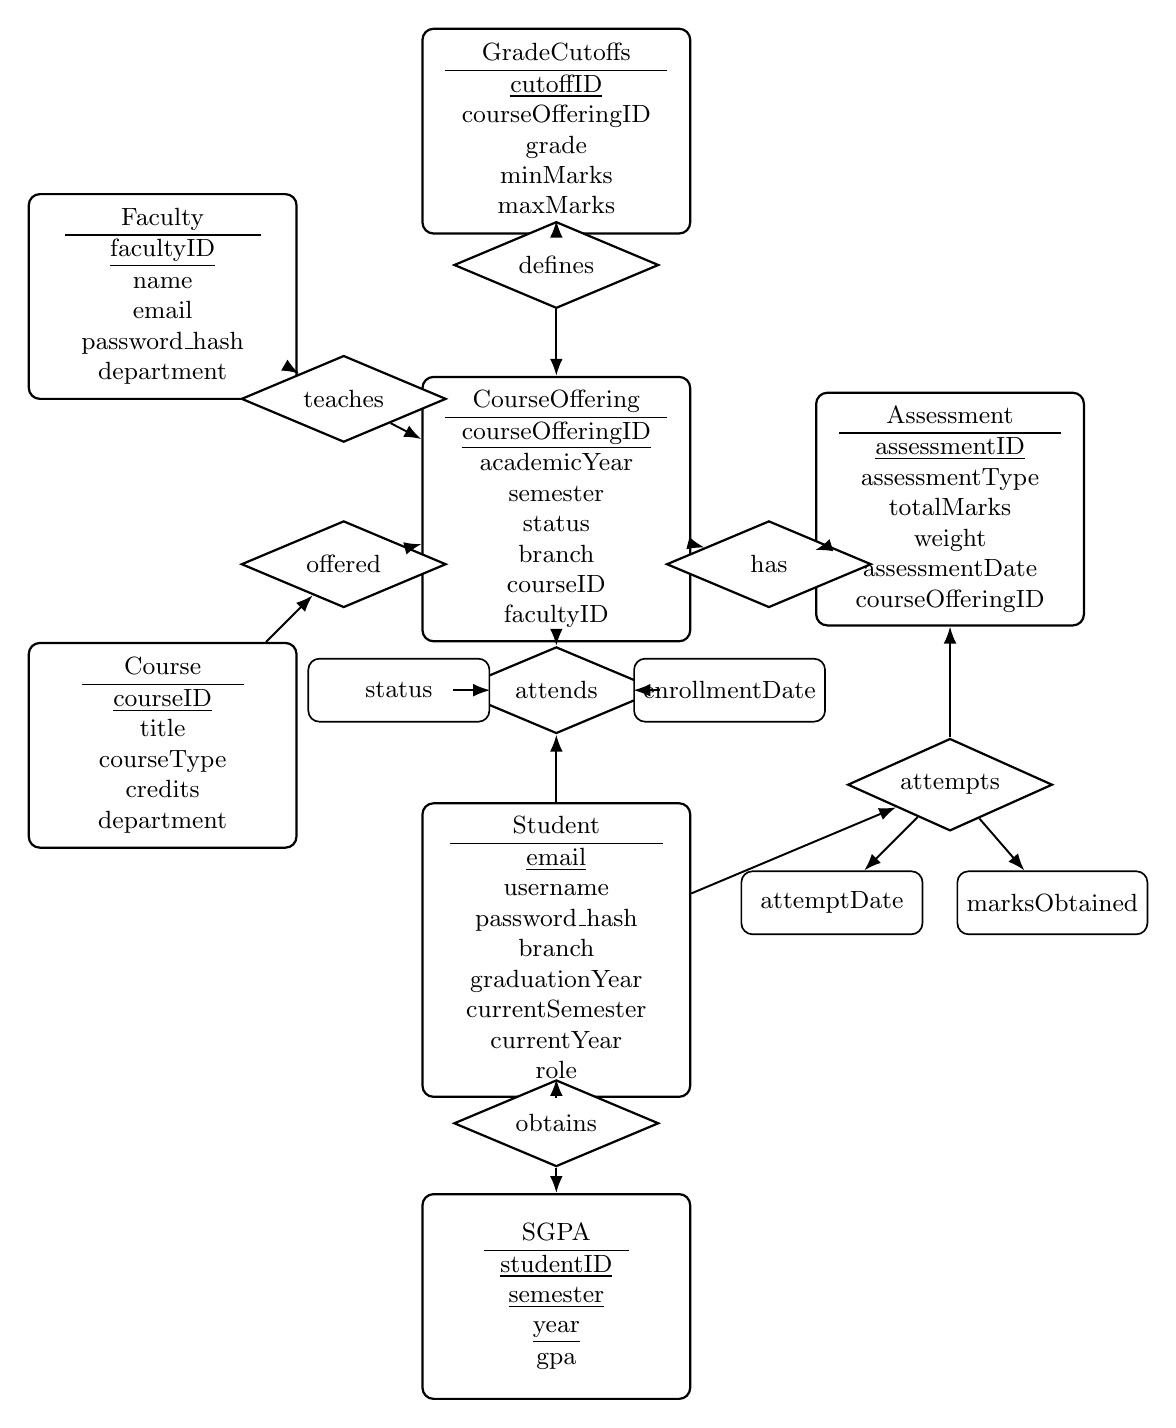
\begin{tikzpicture}[
  entity/.style={draw, rounded corners, minimum width=3.4cm, minimum height=2.6cm, align=center, font=\small, fill=white, line width=0.8pt},
  relationship/.style={draw, diamond, aspect=2.2, minimum width=2.6cm, minimum height=1.1cm, align=center, font=\small, fill=white, line width=0.8pt},
  attribute/.style={draw, rounded corners, minimum width=2.3cm, minimum height=0.8cm, align=center, font=\small, fill=white, line width=0.6pt},
  line/.style={-Latex, line width=0.7pt}
]
  \node[entity] (faculty) at (0,4.5) {\begin{tabular}{c}Faculty\\\hline \pk{facultyID}\\name\\email\\password\_hash\\department\end{tabular}};
  \node[entity] (course) at (0,-1.2) {\begin{tabular}{c}Course\\\hline \pk{courseID}\\title\\courseType\\credits\\department\end{tabular}};
  \node[entity] (offering) at (5,1.8) {\begin{tabular}{c}CourseOffering\\\hline \pk{courseOfferingID}\\academicYear\\semester\\status\\branch\\courseID\\facultyID\end{tabular}};
  \node[entity] (assessment) at (10,1.8) {\begin{tabular}{c}Assessment\\\hline \pk{assessmentID}\\assessmentType\\totalMarks\\weight\\assessmentDate\\courseOfferingID\end{tabular}};
  \node[entity] (gradecut) at (5,6.6) {\begin{tabular}{c}GradeCutoffs\\\hline \pk{cutoffID}\\courseOfferingID\\grade\\minMarks\\maxMarks\end{tabular}};
  \node[entity] (student) at (5,-3.8) {\begin{tabular}{c}Student\\\hline \pk{email}\\username\\password\_hash\\branch\\graduationYear\\currentSemester\\currentYear\\role\end{tabular}};
  \node[entity] (sgpa) at (5,-8.2) {\begin{tabular}{c}SGPA\\\hline \pk{studentID}\\\pk{semester}\\\pk{year}\\gpa\end{tabular}};

  \node[relationship] (teaches) at (2.3,3.2) {teaches};
  \node[relationship] (offers) at (2.3,1.1) {offered};
  \node[relationship] (defines) at (5,4.9) {defines};
  \node[relationship] (has) at (7.7,1.1) {has};
  \node[relationship] (attends) at (5,-0.5) {attends};
  \node[relationship] (attempts) at (10,-1.7) {attempts};
  \node[relationship] (obtains) at (5,-6.0) {obtains};

  \node[attribute] (attstatus) at (3.0,-0.5) {status};
  \node[attribute] (attdate) at (7.2,-0.5) {enrollmentDate};
  \node[attribute] (attemptdate) at (8.5,-3.2) {attemptDate};
  \node[attribute] (marksobt) at (11.3,-3.2) {marksObtained};

  \draw[line] (faculty) -- (teaches);
  \draw[line] (teaches) -- (offering);
  \draw[line] (course) -- (offers);
  \draw[line] (offers) -- (offering);
  \draw[line] (gradecut) -- (defines);
  \draw[line] (defines) -- (offering);
  \draw[line] (offering) -- (has);
  \draw[line] (has) -- (assessment);
  \draw[line] (offering) -- (attends);
  \draw[line] (student) -- (attends);
  \draw[line] (attends) -- (attstatus);
  \draw[line] (attends) -- (attdate);
  \draw[line] (student) -- (obtains);
  \draw[line] (obtains) -- (sgpa);
  \draw[line] (student) -- (attempts);
  \draw[line] (attempts) -- (assessment);
  \draw[line] (attempts) -- (attemptdate);
  \draw[line] (attempts) -- (marksobt);
\end{tikzpicture}}
\caption{Conceptual ER diagram of the Oracle-based performance management system}
\label{fig:er}
\end{figure}

\section{Final Relation Schema}
The implementation uses the following relations in Oracle:
\begin{itemize}[leftmargin=1.5em]
  \item \texttt{STUDENT(email, username, password\_hash, branch, graduation\_year, current\_semester, current\_year, role)}
  \item \texttt{FACULTY(faculty\_id, name, email, password\_hash, department)}
  \item \texttt{COURSE(course\_id, title, course\_type, credits, department)}
  \item \texttt{COURSE\_OFFERING(course\_offering\_id, academic\_year, semester, status, branch, course\_id, faculty\_id)}
  \item \texttt{ASSESSMENT(assessment\_id, assessment\_type, total\_marks, weight, assessment\_date, course\_offering\_id)}
  \item \texttt{GRADE\_CUTOFFS(cutoff\_id, grade, min\_marks, max\_marks, course\_offering\_id)}
  \item \texttt{SGPA(student\_id, semester, academic\_year, gpa)}
  \item \texttt{ATTENDS(student\_mail, course\_offering\_id, enrollment\_date, status, final\_grade)}
  \item \texttt{ATTEMPTS(student\_mail, assessment\_id, attempt\_date, marks\_obtained)}
\end{itemize}

\section{Design Alternatives}
\subsection{Redundancy}
An alternative design could have stored total marks, weighted totals, and final grades in separate summary tables. That design would make reads faster but would duplicate state and complicate updates. The implemented schema keeps raw academic data normalized and computes totals on demand, while storing \texttt{final\_grade} in \texttt{attends} as a controlled denormalization for stable display.

\subsection{Incompleteness}
An incomplete design would omit course-offering status, cutoffs, or persistent enrollment outcomes. The implemented schema includes \texttt{status} in \texttt{course\_offering} and \texttt{final\_grade} in \texttt{attends}, which supports archived offerings and historical grade retrieval.

\subsection{Decomposition}
A poor design would collapse everything into one wide relation such as \texttt{student\_course\_data}. The current decomposition splits entities and transactions into separate tables, reducing duplication and keeping updates local to their owning entity.

\section{Normalization}
\subsection{First Normal Form}
All attributes are atomic. There are no repeating columns such as \texttt{quiz1}, \texttt{quiz2}, or nested lists of marks. The schema is therefore in 1NF.

\subsection{Second Normal Form}
The tables with composite keys, such as \texttt{attends} and \texttt{attempts}, have attributes that depend on the full key. For example, \texttt{(student\_mail, assessment\_id) -> attempt\_date, marks\_obtained}. The schema satisfies 2NF.

\subsection{Third Normal Form}
Non-key attributes are separated into their own relations. Course details are not repeated in course offerings, and assessment details are not repeated in attempts. The schema is in 3NF, with one intentional exception: \texttt{attends.final\_grade} is stored for usability.

\subsection{Boyce-Codd Normal Form}
The functional dependencies in the core relations are key-based, such as \texttt{assessment\_id -> assessment\_type, total\_marks, weight, assessment\_date, course\_offering\_id}. The design is BCNF-oriented, aside from the deliberate stored grade field.

\subsection{Implementation Differences from the Early Sketch}
The early ER sketch used separate relationship tables such as \texttt{HAS}, \texttt{TEACHES}, and \texttt{DEFINES}. In the final implementation, those are represented by foreign keys in \texttt{assessment}, \texttt{course\_offering}, and \texttt{grade\_cutoffs}. The codebase also includes derived views that were not visible in the sketch, namely \texttt{v\_student\_course\_progress} and \texttt{v\_student\_profile}.

\chapter{DDL Commands, PL/SQL Procedures, Functions, and Triggers}

\section{Schema Definition}
The following listing summarizes the Oracle schema used by the project.

\begin{lstlisting}[language=SQL,caption={Core DDL commands}]
CREATE TABLE student (
  email VARCHAR2(255) PRIMARY KEY,
  username VARCHAR2(120) NOT NULL,
  password_hash VARCHAR2(255) NOT NULL,
  branch VARCHAR2(20) NOT NULL,
  graduation_year NUMBER(4) NOT NULL,
  current_semester NUMBER(2) NOT NULL,
  current_year NUMBER(4) NOT NULL,
  role VARCHAR2(20) DEFAULT 'student' NOT NULL
);

CREATE TABLE faculty (
  faculty_id NUMBER GENERATED BY DEFAULT AS IDENTITY PRIMARY KEY,
  name VARCHAR2(120) NOT NULL,
  email VARCHAR2(255) NOT NULL UNIQUE,
  password_hash VARCHAR2(255) NOT NULL,
  department VARCHAR2(20) NOT NULL
);

CREATE TABLE course_offering (
  course_offering_id NUMBER GENERATED BY DEFAULT AS IDENTITY PRIMARY KEY,
  academic_year NUMBER(4) NOT NULL,
  semester NUMBER(2) NOT NULL,
  status VARCHAR2(20) DEFAULT 'current' NOT NULL,
  branch VARCHAR2(20) NOT NULL,
  course_id VARCHAR2(20) NOT NULL,
  faculty_id NUMBER NOT NULL,
  CONSTRAINT fk_course_offering_course FOREIGN KEY (course_id) REFERENCES course(course_id),
  CONSTRAINT fk_course_offering_faculty FOREIGN KEY (faculty_id) REFERENCES faculty(faculty_id)
);

CREATE TABLE assessment (
  assessment_id NUMBER GENERATED BY DEFAULT AS IDENTITY PRIMARY KEY,
  assessment_type VARCHAR2(60) NOT NULL,
  total_marks NUMBER(4) NOT NULL,
  weight NUMBER(5,2) NOT NULL,
  assessment_date DATE DEFAULT SYSDATE NOT NULL,
  course_offering_id NUMBER NOT NULL,
  CONSTRAINT fk_assessment_course_offering FOREIGN KEY (course_offering_id)
    REFERENCES course_offering(course_offering_id)
);

CREATE TABLE grade_cutoffs (
  cutoff_id NUMBER GENERATED BY DEFAULT AS IDENTITY PRIMARY KEY,
  grade VARCHAR2(3) NOT NULL,
  min_marks NUMBER(5,2) NOT NULL,
  max_marks NUMBER(5,2) NOT NULL,
  course_offering_id NUMBER NOT NULL,
  CONSTRAINT fk_cutoff_course_offering FOREIGN KEY (course_offering_id)
    REFERENCES course_offering(course_offering_id)
);

CREATE TABLE attends (
  student_mail VARCHAR2(255) NOT NULL,
  course_offering_id NUMBER NOT NULL,
  enrollment_date DATE NOT NULL,
  status VARCHAR2(20) NOT NULL,
  final_grade VARCHAR2(3),
  CONSTRAINT pk_attends PRIMARY KEY (student_mail, course_offering_id),
  CONSTRAINT fk_attends_student FOREIGN KEY (student_mail) REFERENCES student(email),
  CONSTRAINT fk_attends_course_offering FOREIGN KEY (course_offering_id)
    REFERENCES course_offering(course_offering_id)
);
\end{lstlisting}

\section{Sample Data}
The seeded dataset in the workspace follows the same structure and can be reproduced with the reset script. The data includes multiple faculty members, students across branches, course offerings for different semesters, assessments with varying weights, and attempts for enrolled students.

\section{Important Queries}
\subsection{Compute Weighted Total Marks}
\begin{lstlisting}[language=SQL]
SELECT
  a.student_mail,
  SUM((a.marks_obtained / b.total_marks) * b.weight) AS total_score
FROM attempts a
JOIN assessment b ON a.assessment_id = b.assessment_id
GROUP BY a.student_mail;
\end{lstlisting}

\subsection{Assign Grades}
\begin{lstlisting}[language=SQL]
SELECT
  t.student_mail,
  t.total_score,
  g.grade
FROM (
  SELECT
    a.student_mail,
    SUM((a.marks_obtained / b.total_marks) * b.weight) AS total_score
  FROM attempts a
  JOIN assessment b ON a.assessment_id = b.assessment_id
  GROUP BY a.student_mail
) t
JOIN grade_cutoffs g
  ON t.total_score BETWEEN g.min_marks AND g.max_marks;
\end{lstlisting}

\subsection{Class Performance Report}
\begin{lstlisting}[language=SQL]
SELECT
  AVG(marks_obtained) AS average,
  MAX(marks_obtained) AS highest,
  MIN(marks_obtained) AS lowest
FROM attempts;
\end{lstlisting}

\section{Functions and Procedures}
\subsection{GetGrade Function}
\begin{lstlisting}[language=SQL]
CREATE OR REPLACE FUNCTION GetGrade(
  p_score NUMBER,
  p_course_offering_id NUMBER
) RETURN VARCHAR2
IS
  v_grade VARCHAR2(3);
BEGIN
  SELECT grade
    INTO v_grade
    FROM grade_cutoffs
   WHERE p_score BETWEEN min_marks AND max_marks
     AND course_offering_id = p_course_offering_id
   ORDER BY min_marks DESC
   FETCH FIRST 1 ROW ONLY;

  RETURN v_grade;
EXCEPTION
  WHEN NO_DATA_FOUND THEN
    RETURN 'F';
END;
\end{lstlisting}

\subsection{GetTotalMarks Procedure}
\begin{lstlisting}[language=SQL]
CREATE OR REPLACE PROCEDURE GetTotalMarks(
  p_student IN VARCHAR2,
  p_total OUT NUMBER
)
IS
BEGIN
  SELECT NVL(ROUND(SUM((at.marks_obtained / NULLIF(asmt.total_marks, 0)) * asmt.weight), 2), 0)
    INTO p_total
    FROM attempts at
    JOIN assessment asmt ON asmt.assessment_id = at.assessment_id
   WHERE at.student_mail = p_student;
END;
/
\end{lstlisting}

\subsection{ClassReport Procedure}
\begin{lstlisting}[language=SQL]
CREATE OR REPLACE PROCEDURE ClassReport(
  p_course_offering_id IN NUMBER,
  p_average OUT NUMBER,
  p_highest OUT NUMBER,
  p_lowest OUT NUMBER
)
IS
BEGIN
  SELECT NVL(ROUND(AVG(at.marks_obtained), 2), 0),
         NVL(MAX(at.marks_obtained), 0),
         NVL(MIN(at.marks_obtained), 0)
    INTO p_average, p_highest, p_lowest
    FROM attempts at
    JOIN assessment asmt ON asmt.assessment_id = at.assessment_id
   WHERE asmt.course_offering_id = p_course_offering_id;
END;
/
\end{lstlisting}

\section{Triggers}
\subsection{Validate Assessment Weight}
\begin{lstlisting}[language=SQL]
CREATE OR REPLACE TRIGGER check_weight
FOR INSERT OR UPDATE ON assessment
COMPOUND TRIGGER
  TYPE t_course_ids IS TABLE OF NUMBER INDEX BY PLS_INTEGER;
  g_course_ids t_course_ids;
  g_index PLS_INTEGER := 0;

  BEFORE EACH ROW IS
  BEGIN
    g_index := g_index + 1;
    g_course_ids(g_index) := :NEW.course_offering_id;
  END BEFORE EACH ROW;

  AFTER STATEMENT IS
    v_total NUMBER;
  BEGIN
    FOR i IN 1 .. g_index LOOP
      SELECT NVL(SUM(weight), 0)
        INTO v_total
        FROM assessment
       WHERE course_offering_id = g_course_ids(i);

      IF v_total > 100 THEN
        RAISE_APPLICATION_ERROR(-20002, 'Total assessment weight exceeds 100');
      END IF;
    END LOOP;
  END AFTER STATEMENT;
END;
/
\end{lstlisting}

\subsection{Validate Marks Range}
\begin{lstlisting}[language=SQL]
CREATE OR REPLACE TRIGGER check_marks
BEFORE INSERT OR UPDATE ON attempts
FOR EACH ROW
DECLARE
  v_max NUMBER;
BEGIN
  SELECT total_marks
    INTO v_max
    FROM assessment
   WHERE assessment_id = :NEW.assessment_id;

  IF :NEW.marks_obtained < 0 OR :NEW.marks_obtained > v_max THEN
    RAISE_APPLICATION_ERROR(-20001, 'Marks exceed the maximum allowed for this assessment');
  END IF;
END;
/
\end{lstlisting}

\section{Derived Views Used by the Application}
The application reads student progress through views rather than computing every presentation query in the UI.
\begin{lstlisting}[language=SQL]
CREATE OR REPLACE VIEW v_student_course_progress AS
SELECT
  a.student_mail,
  fo.course_offering_id,
  fo.academic_year,
  fo.semester,
  fo.branch,
  c.course_id,
  c.title AS course_title,
  c.course_type,
  c.credits,
  f.name AS faculty_name,
  NVL((
    SELECT ROUND(SUM(at.marks_obtained), 2)
    FROM attempts at
    JOIN assessment asmt ON asmt.assessment_id = at.assessment_id
    WHERE at.student_mail = a.student_mail
      AND asmt.course_offering_id = fo.course_offering_id
  ), 0) AS earned_raw,
  NVL((
    SELECT ROUND(SUM(asmt.total_marks), 2)
    FROM attempts at
    JOIN assessment asmt ON asmt.assessment_id = at.assessment_id
    WHERE at.student_mail = a.student_mail
      AND asmt.course_offering_id = fo.course_offering_id
  ), 0) AS possible_raw,
  NVL((
    SELECT ROUND(SUM((at.marks_obtained / NULLIF(asmt.total_marks, 0)) * asmt.weight), 2)
    FROM attempts at
    JOIN assessment asmt ON asmt.assessment_id = at.assessment_id
    WHERE at.student_mail = a.student_mail
      AND asmt.course_offering_id = fo.course_offering_id
  ), 0) AS weighted_total,
  a.final_grade,
  a.status AS status
FROM attends a
JOIN course_offering fo ON fo.course_offering_id = a.course_offering_id
JOIN course c ON c.course_id = fo.course_id
JOIN faculty f ON f.faculty_id = fo.faculty_id;
\end{lstlisting}

\chapter{Conclusion, Limitations, and Future Work}
The project demonstrates how Oracle SQL and PL/SQL can support a realistic academic workflow without hardcoded assessment columns. The implemented schema satisfies the main requirements for dynamic assessments, computed totals, grading cutoffs, data validation, and report generation.

The primary limitation is that the current implementation stores one attempt per student per assessment and relies on application logic to refresh final grades after changes. A future enhancement could add multi-attempt support, audit history for cutoff changes, and automatic refresh mechanisms for derived grade summaries. Another useful extension would be a richer analytics layer for section-wise performance comparison and transcript generation.

\chapter{References}
\begin{thebibliography}{9}
\bibitem{elmasri}
R. Elmasri and S. B. Navathe, \textit{Fundamentals of Database Systems}, Pearson.

\bibitem{oracle}
Oracle Corporation, \textit{Oracle Database SQL Language Reference}.

\bibitem{plsql}
Oracle Corporation, \textit{PL/SQL Language Reference}.

\bibitem{next}
Next.js Documentation, \textit{https://nextjs.org/docs}.
\end{thebibliography}

\end{document}